\begin{frame}
  \frametitle{Kernel Development News}
  \begin{itemize}
  \item Linux Weekly News
    \begin{itemize}
    \item \url{http://lwn.net/}
    \item The weekly digest off all Linux and free software
      information sources
    \item In depth technical discussions about the kernel
    \item Subscribe to finance the editors (\$7 / month)
    \item Articles available for non subscribers after 1 week.
    \end{itemize}
  \end{itemize}
\end{frame}

\begin{frame}
  \frametitle{Useful Reading (1)}
  \begin{columns}
    \column{0.7\textwidth}
    \begin{itemize}
    \item Essential Linux Device Drivers, April 2008
      \begin{itemize}
      \item \url{http://free-electrons.com/redirect/eldd-book.html}
      \item By Sreekrishnan Venkateswaran, an embedded IBM engineer
        with more than 10 years of experience
      \item Covers a wide range of topics not covered by LDD: serial
        drivers, input drivers, I2C, PCMCIA and Compact Flash, PCI,
        USB, video drivers, audio drivers, block drivers, network
        drivers, Bluetooth, IrDA, MTD, drivers in userspace, kernel
        debugging, etc.
      \item \emph{Probably the most wide ranging and complete Linux
          device driver book I've read} -- Alan Cox
      \end{itemize}
    \end{itemize}
    \column{0.3\textwidth}
    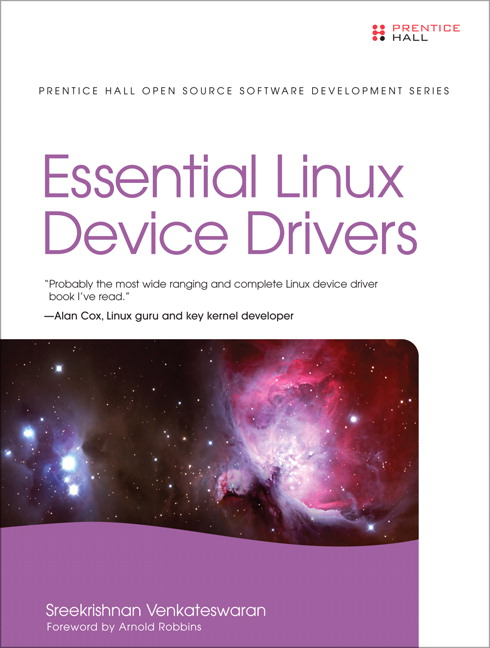
\includegraphics[width=\textwidth]{slides/kernel-resources-references/eldd.jpg}
  \end{columns}
\end{frame}

\begin{frame}
  \frametitle{Useful Reading (2)}
  \begin{columns}
    \column{0.7\textwidth}
    \begin{itemize}
    \item Writing Linux Device drivers, September 2009
      \begin{itemize}
      \item \url{http://www.coopj.com/}
      \item Self published by Jerry Cooperstein
      \item Available like any other book (Amazon and others)
      \item Though not as thorough as the previous book on specific
        drivers, still a good complement on multiple aspects of kernel
        and device driver development.
      \item Based on Linux 2.6.31
      \item Multiple exercises. Updated solutions for 2.6.36.
      \end{itemize}
    \end{itemize}
    \column{0.3\textwidth}
    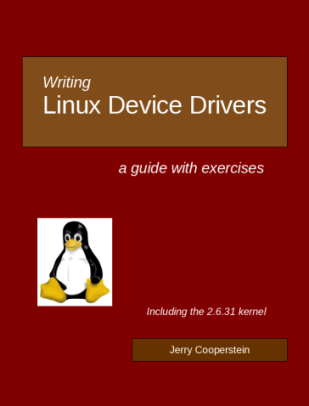
\includegraphics[width=\textwidth]{slides/kernel-resources-references/writing-linux-device-drivers.png}
  \end{columns}
\end{frame}

\begin{frame}
  \frametitle{Useful Reading (3)}
  \begin{columns}
    \column{0.7\textwidth}
    \begin{itemize}
    \item Linux Device Drivers, 3rd edition, Feb 2005
      \begin{itemize}
      \item \url{http://www.oreilly.com/catalog/linuxdrive3/}
      \item By Jonathan Corbet, Alessandro Rubini, Greg Kroah-Hartman,
        O'Reilly
      \item Freely available on-line! Great companion to the printed
        book for easy electronic searches!
      \item \url{http://lwn.net/Kernel/LDD3/} (1 PDF file per chapter)
      \item \url{http://free-electrons.com/community/kernel/ldd3/}
        (single PDF file)
      \item Getting outdated but still useful for Linux device driver
        writers!
      \end{itemize}
    \end{itemize}
    \column{0.3\textwidth}
    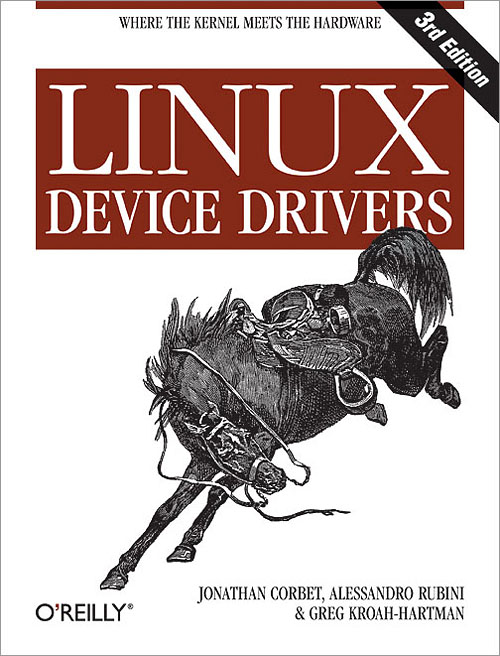
\includegraphics[width=\textwidth]{slides/kernel-resources-references/linux-device-drivers.jpg}
  \end{columns}
\end{frame}

\begin{frame}
  \frametitle{Useful Reading (4)}
  \begin{columns}
    \column{0.7\textwidth}
    \begin{itemize}
    \item Linux Kernel Development, 3rd Edition, Jun 2010
      \begin{itemize}
      \item Robert Love, Novell Press
      \item \url{http://free-electrons.com/redir/lkd3-book.html}
      \item A very synthetic and pleasant way to learn about kernel
        subsystems (beyond the needs of device driver writers)
      \end{itemize}
    \item The Linux Programming Interface, Oct 2010
      \begin{itemize}
      \item Michael Kerrisk, No Starch Press
      \item \url{http://man7.org/tlpi/}
      \item A gold mine about the kernel interface and how to use it
      \end{itemize}
    \end{itemize}
    \column{0.3\textwidth}
    \begin{center}
      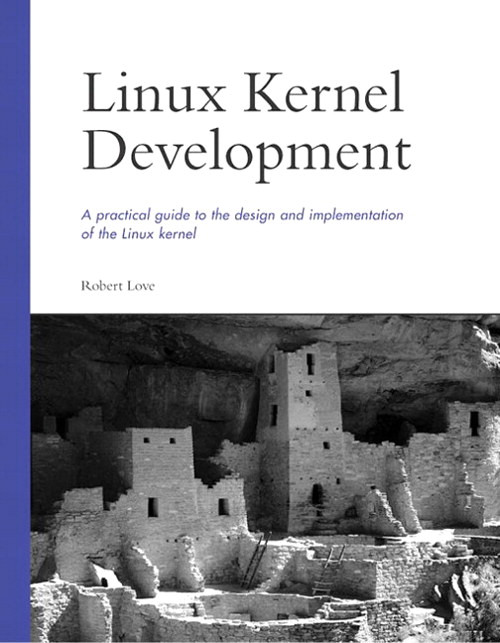
\includegraphics[height=0.4\textheight]{slides/kernel-resources-references/linux-kernel-development.jpg}\\
      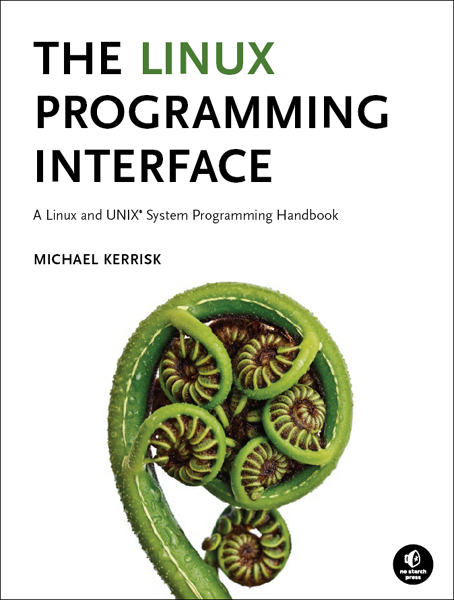
\includegraphics[height=0.4\textheight]{slides/kernel-resources-references/linux-programming-interface.png}
    \end{center}
  \end{columns}
\end{frame}

\begin{frame}
  \frametitle{Useful Online Resources}
  \begin{itemize}
  \item Kernel documentation (\code{Documentation/} in kernel sources)
    \begin{itemize}
    \item Available on line:
      \url{http://free-electrons.com/kerneldoc/} (with HTML
      documentation extracted from source code)
    \end{itemize}
  \item Linux kernel mailing list FAQ
    \begin{itemize}
    \item \url{http://www.tux.org/lkml/}
    \item Complete Linux kernel FAQ
    \item Read this before asking a question to the mailing list
    \end{itemize}
  \item Kernel Newbies
    \begin{itemize}
    \item \url{http://kernelnewbies.org/}
    \item Glossary, articles, presentations, HOWTOs, recommended
      reading, useful tools for people getting familiar with Linux
      kernel or driver development.
    \end{itemize}
  \item Kernel glossary
    \begin{itemize}
    \item \url{http://kernelnewbies.org/KernelGlossary}
    \end{itemize}
\end{itemize}

\end{frame}

\begin{frame}
  \frametitle{International Conferences}
  \begin{itemize}
  \item Embedded Linux Conference: \url{http://embeddedlinuxconference.com/}
    \begin{itemize}
    \item Organized by the CE Linux Forum:
    \item in California (San Francisco, April)
    \item in Europe (October-November)
    \item Very interesting kernel and userspace topics for embedded
      systems developers.
    \item Presentation slides freely available
    \end{itemize}
  \item Linux Plumbers: \url{http://linuxplumbersconf.org}
    \begin{itemize}
    \item Conference on the low-level plumbing of Linux: kernel,
      audio, power management, device management, multimedia, etc.
    \end{itemize}
  \item linux.conf.au: \url{http://linux.org.au/conf/}
    \begin{itemize}
    \item In Australia / New Zealand
    \item Features a few presentations by key kernel hackers.
    \end{itemize}
  \item Don't miss our free conference videos on
    \url{http://free-electrons.com/community/videos/conferences/}
  \end{itemize}
\end{frame}

\begin{frame}
  \frametitle{ARM resources}
  \begin{itemize}
  \item ARM Linux project: \url{http://www.arm.linux.org.uk/}
    \begin{itemize}
    \item Developer documentation:
      \url{http://www.arm.linux.org.uk/developer/}
    \item linux-arm-kernel mailing list:
      \url{http://lists.infradead.org/mailman/listinfo/linux-arm-kernel}
    \item FAQ: \url{http://www.arm.linux.org.uk/armlinux/mlfaq.php}
    \end{itemize}
  \item Linaro: \url{http://linaro.org}
    \begin{itemize}
    \item Many optimizations and resources for recent ARM CPUs
      (toolchains, kernels, debugging utilities...).
    \end{itemize}
  \item ARM Limited: \url{http://www.linux-arm.com/}
    \begin{itemize}
    \item Wiki with links to useful developer resources
    \end{itemize}
  \item See our Embedded Linux course for details about toolchains:
    {\small
     \url{http://free-electrons.com/training/embedded-linux/}}
  \end{itemize}
\end{frame}
